\documentclass[12pt,a4paper]{report}

% ─── Packages ───────────────────────────────────────────────────────────────
\usepackage[a4paper, margin=1in]{geometry}
\usepackage{times}
\usepackage{setspace}
\usepackage{graphicx}
\usepackage{amsmath, amssymb}
\usepackage{booktabs}
\usepackage{array}
\usepackage{longtable}
\usepackage{hyperref}
\usepackage{url}
\usepackage{cite}
\usepackage{caption}
\usepackage{subcaption}
\usepackage{float}
\usepackage{listings}
\usepackage{xcolor}
\usepackage{fancyhdr}
\usepackage{titlesec}
\usepackage{tocloft}
\usepackage{enumitem}
\usepackage{tikz}
\usepackage{pgfplots}
\usepackage{pgfplotstable}
\pgfplotsset{compat=1.18}
\usepackage{multirow}
\usepackage{tabularx}
\usepackage[acronym]{glossaries}
\usepackage{parskip}

% TikZ libraries needed for all diagrams
\usetikzlibrary{
  shapes.geometric, shapes.misc, shapes.arrows,
  arrows.meta, positioning, fit, calc,
  decorations.pathreplacing, backgrounds, shadows,
  patterns
}

% ─── Hyperref Setup ─────────────────────────────────────────────────────────
\hypersetup{
    colorlinks=true,
    linkcolor=blue!70!black,
    citecolor=green!50!black,
    urlcolor=blue!70!black,
    pdftitle={Wind DSM Optimization: Physics-Informed Predictive Machine Learning},
    pdfauthor={Tapas Barman},
}

% ─── Header / Footer ────────────────────────────────────────────────────────
\pagestyle{fancy}
\fancyhf{}
\fancyhead[L]{\small Wind DSM Optimization: PI-PML}
\fancyhead[R]{\small IIIT Lucknow}
\fancyfoot[C]{\thepage}
\renewcommand{\headrulewidth}{0.4pt}

% ─── Chapter Title Formatting ───────────────────────────────────────────────
\titleformat{\chapter}[display]
  {\normalfont\huge\bfseries}{\chaptertitlename\ \thechapter}{20pt}{\Huge}
\titlespacing*{\chapter}{0pt}{30pt}{20pt}

% ─── Listings Style ─────────────────────────────────────────────────────────
\lstset{
  basicstyle=\ttfamily\small,
  keywordstyle=\color{blue}\bfseries,
  commentstyle=\color{gray},
  stringstyle=\color{red!70!black},
  breaklines=true,
  frame=single,
  numbers=left,
  numberstyle=\tiny\color{gray},
  captionpos=b,
}

% ─── Colour palette used across all TikZ diagrams ───────────────────────────
\definecolor{physblue}{RGB}{31,119,180}
\definecolor{mlgreen}{RGB}{44,160,44}
\definecolor{dsmred}{RGB}{214,39,40}
\definecolor{mlflow}{RGB}{255,127,14}
\definecolor{apigray}{RGB}{127,127,127}
\definecolor{lightbg}{RGB}{240,248,255}
\definecolor{darkbg}{RGB}{30,30,50}

% ─── Acronyms ───────────────────────────────────────────────────────────────
\makeglossaries
\newacronym{piml}{PI-PML}{Physics-Informed Predictive Machine Learning}
\newacronym{dsm}{DSM}{Deviation Settlement Mechanism}
\newacronym{cerc}{CERC}{Central Electricity Regulatory Commission}
\newacronym{gfs}{GFS}{Global Forecast System}
\newacronym{noaa}{NOAA}{National Oceanic and Atmospheric Administration}
\newacronym{srpc}{SRPC}{Southern Regional Power Committee}
\newacronym{scada}{SCADA}{Supervisory Control and Data Acquisition}
\newacronym{pchip}{PCHIP}{Piecewise Cubic Hermite Interpolating Polynomial}
\newacronym{idw}{IDW}{Inverse Distance Weighting}
\newacronym{dfig}{DFIG}{Doubly-Fed Induction Generator}
\newacronym{mae}{MAE}{Mean Absolute Error}
\newacronym{rmse}{RMSE}{Root Mean Square Error}
\newacronym{nwp}{NWP}{Numerical Weather Prediction}
\newacronym{mlops}{MLOps}{Machine Learning Operations}
\newacronym{api}{API}{Application Programming Interface}
\newacronym{acp}{ACP}{Area Clearing Price}

%=============================================================================
\begin{document}
%=============================================================================

% ─── PAGE 1: Title Page ───────────────────────────────────────────────────────
\begin{titlepage}
  \thispagestyle{empty}
  \centering
  \vspace*{3cm}

  {\Large\bfseries Wind DSM Optimization: Physics-Informed\\[0.4cm]
   Predictive Machine Learning (PI-PML)\\[1.2cm]}

  \textit{A thesis submitted in partial fulfillment of the requirements for the award of the\\
  degree of}\\[1cm]

  {\large\bfseries MSc.}\\[0.1cm]
  in\\[0.1cm]
  {\large\bfseries Data Science}\\[1.2cm]

  by\\[0.5cm]

  {\large\bfseries Tapas Barman}\\[0.1cm]
  {\large (Roll Number: MSD24021)}\\[1.2cm]

  under the guidance of\\[0.5cm]

  {\large\bfseries Dr.\ Sirsendu Sekhar Barman}\\[1.5cm]

  % Place iiitl_logo.png in the same folder to render the logo
  
\includegraphics[width=0.22\textwidth]{iiitl_logo.png}\\[0.8cm]

  {\large\bfseries Indian Institute of Information Technology, Lucknow}\\[0.1cm]
  {\large 2024-26}\\[0.4cm]

  {\small \textcopyright\ Indian Institute of Information Technology, Lucknow 2025.}
\end{titlepage}

% ─── PAGE 2: Certificate ─────────────────────────────────────────────────────
\setcounter{page}{1}
\thispagestyle{plain}

\chapter*{\Huge\bfseries CERTIFICATE}
\addcontentsline{toc}{chapter}{Certificate}

\noindent This is to certify that the thesis entitled
\textbf{``Wind DSM Optimization: Physics-Informed Predictive Machine Learning (PI-PML)''}
submitted by \textbf{Tapas Barman} who got his name registered on \textbf{Jul 2024} for
the award of M.Sc degree at Indian Institute of Information Technology, Lucknow is
absolutely based upon his own work under the supervision of
\textbf{Dr.\ Sirsendu Sekhar Barman}, Department of Mathematics, Indian Institute of
Information Technology, Lucknow -- 226\,002, U.P., India and that neither this thesis nor
any part of it has been submitted for any degree or any other academic award anywhere before.

\vspace{3.5cm}

\noindent
\begin{minipage}[t]{0.5\textwidth}
  Dr.\ Sirsendu Sekhar Barman\\
  Department of Mathematics\\
  Indian Institute of Information Technol-\\
  ogy\\
  Pin -- 226002, INDIA
\end{minipage}%
\hfill
\begin{minipage}[t]{0.42\textwidth}
  \vspace{0pt}
  \rule{6cm}{0.4pt}\\[0.15cm]
  \hfill Supervisor Signature
\end{minipage}

\newpage

% ─── PAGE 3: Authorship ───────────────────────────────────────────────────────
\thispagestyle{plain}

\chapter*{\Huge\bfseries AUTHORSHIP}
\addcontentsline{toc}{chapter}{Authorship}

\noindent I, \textbf{Tapas Barman}, declare that this thesis titled,
\textbf{``Wind DSM Optimization: Physics-Informed Predictive Machine Learning (PI-PML)''}
and the work presented in it are my own. I confirm that:

\vspace{0.5cm}

\begin{itemize}[leftmargin=1.5em, itemsep=0.5em]
  \item This work was completed entirely while in candidature for Master of Science
        degree at Indian Institute of Information Technology, Lucknow.
  \item Where I have consulted the published work of others, it is always cited.
  \item Wherever I have cited the work of others, the source is always indicated. Except
        for the aforementioned quotations, this thesis is solely my work.
  \item I have acknowledged all major sources of information.
\end{itemize}

\vspace{2cm}
\noindent\textbf{Signature:}\\[1cm]
\rule{4.5cm}{0.4pt}
\vspace{1cm}

\noindent\textbf{Date: 29-05-2026}

% ─── Acknowledgements ────────────────────────────────────────────────────────
\chapter*{Acknowledgements}
\addcontentsline{toc}{chapter}{Acknowledgements}

First and foremost, I would like to express my sincere gratitude to my supervisor,
\textbf{Dr.\ Sirsendu Sekhar Barman}, for his continuous support, expert guidance, and
encouragement throughout the course of this project. His deep insights into machine learning,
power systems, and applied mathematics have been invaluable in shaping the direction and
quality of this work.

I am also thankful to all the faculty members and staff of the Mathematics Department,
IIIT Lucknow, for providing a stimulating academic environment and the necessary facilities
to carry out this research.

I extend my heartfelt thanks to my friends and classmates for their constructive discussions,
moral support, and cooperation. Finally, I am deeply indebted to my family for their
unconditional love, patience, and constant encouragement, which have always been a source
of strength and inspiration.

\vspace{1.5cm}
\begin{flushright}
  \textbf{Tapas Barman}\\
  MSD24021
\end{flushright}

% ─── Abstract ────────────────────────────────────────────────────────────────
\chapter*{Abstract}
\addcontentsline{toc}{chapter}{Abstract}
\onehalfspacing

Wind energy forecasting inaccuracies impose substantial financial penalties on plant operators
in India under the \gls{cerc} \gls{dsm} framework, which enforces strict 15-minute block
scheduling with penalty bands of 10--15\%. This report presents the design, implementation,
and validation of a \textbf{Double-Engine Forecasting Pipeline} built on \gls{piml}, which
substantially reduces grid deviation penalties for wind power plant operators.

The architecture combines a \textbf{deterministic physics baseline} (Vestas~V112 turbine
aerodynamics modelled via \texttt{windpowerlib}) with a \textbf{stochastic residual learner}
(XGBoost) that predicts the systematic error of the physics engine caused by local terrain,
atmospheric humidity, and diurnal patterns. Live weather data is obtained from the NOAA
NOMADS \gls{gfs}, spatially downscaled from 25~km to 1~km resolution using bilinear spline
interpolation with logarithmic wind-profile corrections, and temporally refined to the
mandatory 96-block, 15-minute grid schedule via \gls{pchip} interpolation.

The pipeline was validated against 29,568 official \gls{srpc} dispatch blocks covering
10 continuous months for the \textbf{75~MW RSOPL Koppal} wind plant in Karnataka. On the
held-out 2-month test set, the PI-PML system reduced Mean Absolute Error by \textbf{71.2\%}
relative to the physics baseline, cutting estimated CERC penalty charges from
\textnumero{}24,83,254 to \textnumero{}1,29,282 --- a saving of approximately
\textbf{\textnumero{}23.5~Lakhs} in two months, projecting to \textbf{\textnumero{}1.41~Crores
per year}.

\vspace{0.5cm}
\noindent\textbf{Keywords:} Wind power forecasting, Physics-Informed Machine Learning,
Deviation Settlement Mechanism, XGBoost residual learning, CERC penalty, NOAA GFS,
spatial downscaling, PCHIP interpolation, MLflow, Champion-Challenger, FastAPI.

\tableofcontents
\listoffigures
\listoftables
\printglossary[type=\acronymtype, title=List of Abbreviations]
\addcontentsline{toc}{chapter}{List of Abbreviations}

%=============================================================================
\chapter{Introduction}
%=============================================================================
\onehalfspacing

\section{Background and Motivation}

India's electricity grid operates under a stringent real-time scheduling regime managed by
the \gls{cerc}. Under the \gls{dsm} regulations, every generator is required to submit a
day-ahead 96-block generation schedule in 15-minute intervals. Any deviation from the
declared schedule attracts financial penalties that escalate in a tiered structure based on the
percentage deviation relative to the plant's Available Capacity (\textit{AvC}).

Wind power plants are inherently vulnerable to DSM penalties because wind speed is
stochastic by nature. A forecast error of even 15--20\% at hub height can push a 75~MW plant
into the highest penalty slab, incurring costs of \textnumero{}1.50 per unit of deviation.

% ══════════════════════════════════════════════════════════════════════════════
% DIAGRAM 1 — DSM Penalty Tier Bar Chart
% Placed here: end of Section 1.1, after explaining the penalty tiers.
% Shows visually how penalties escalate across the three deviation bands.
% ══════════════════════════════════════════════════════════════════════════════
\begin{figure}[H]
  \centering
  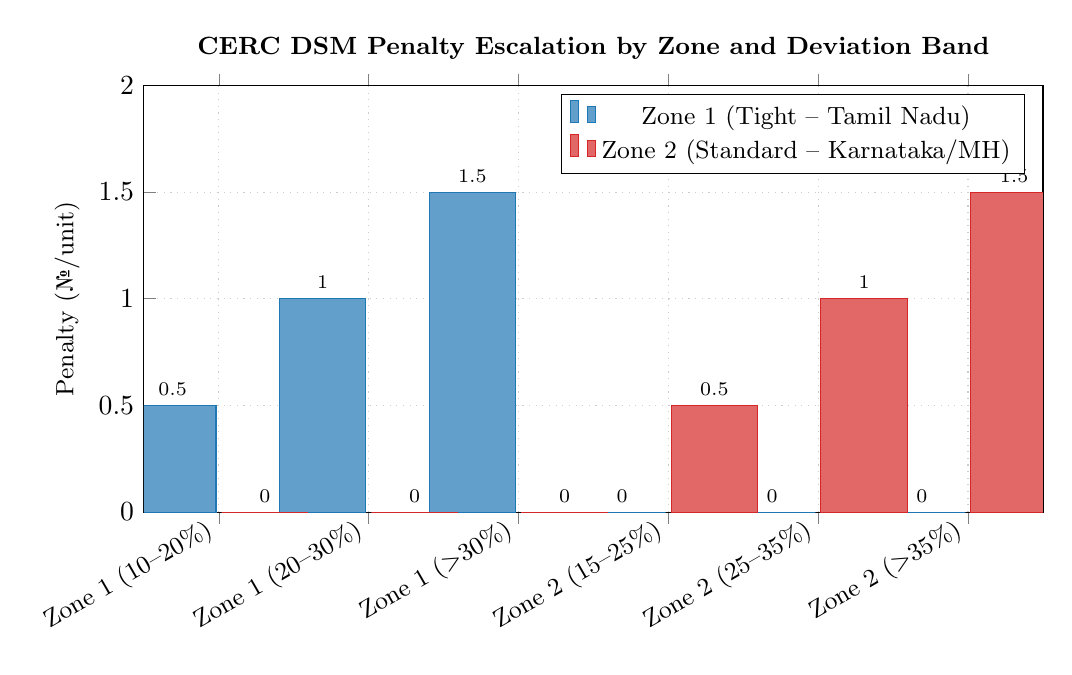
\begin{tikzpicture}
    \begin{axis}[
      ybar,
      bar width=1.1cm,
      width=13cm, height=7cm,
      symbolic x coords={Zone 1 (10--20\%), Zone 1 (20--30\%), Zone 1 ($>$30\%),
                         Zone 2 (15--25\%), Zone 2 (25--35\%), Zone 2 ($>$35\%)},
      xtick=data,
      x tick label style={rotate=30, anchor=east, font=\small},
      ymin=0, ymax=2,
      ylabel={Penalty (\textnumero{}/unit)},
      ylabel style={font=\small},
      title={CERC DSM Penalty Escalation by Zone and Deviation Band},
      title style={font=\small\bfseries},
      nodes near coords,
      nodes near coords style={font=\scriptsize},
      grid=major,
      grid style={dotted, gray!40},
      legend style={at={(0.98,0.98)}, anchor=north east, font=\small},
    ]
      \addplot[fill=physblue!70, draw=physblue]
        coordinates {
          (Zone 1 (10--20\%), 0.50)
          (Zone 1 (20--30\%), 1.00)
          (Zone 1 ($>$30\%),  1.50)
          (Zone 2 (15--25\%), 0)
          (Zone 2 (25--35\%), 0)
          (Zone 2 ($>$35\%),  0)
        };
      \addplot[fill=dsmred!70, draw=dsmred]
        coordinates {
          (Zone 1 (10--20\%), 0)
          (Zone 1 (20--30\%), 0)
          (Zone 1 ($>$30\%),  0)
          (Zone 2 (15--25\%), 0.50)
          (Zone 2 (25--35\%), 1.00)
          (Zone 2 ($>$35\%),  1.50)
        };
      \legend{Zone 1 (Tight -- Tamil Nadu), Zone 2 (Standard -- Karnataka/MH)}
    \end{axis}
  \end{tikzpicture}
  \caption{CERC DSM penalty escalation across deviation bands for Zone~1 and Zone~2.
           The tiered structure motivates accurate forecasting to stay within the free band.}
  \label{fig:dsm_penalty_tiers}
\end{figure}
% ══════════════════════════════════════════════════════════════════════════════

\section{Problem Statement}

\begin{quote}
\textit{How can wind power operators in India significantly reduce their CERC DSM penalty
liability through more accurate day-ahead 96-block generation forecasts, using a combination
of physics-based turbine modelling and data-driven machine learning?}
\end{quote}

\section{Research Objectives}

\begin{enumerate}
  \item Design and implement a PI-PML pipeline combining a deterministic turbine physics
        baseline with an XGBoost residual correction model.
  \item Implement spatially and temporally consistent weather downscaling from NOAA GFS
        25~km grids to the 1~km plant coordinate at hub height.
  \item Accurately simulate the CERC DSM penalty structure across all three regulatory zones.
  \item Implement a production-grade MLOps lifecycle using MLflow with a
        Champion-Challenger model promotion framework.
  \item Validate the system against real official SRPC dispatch data for the RSOPL Koppal
        75~MW wind plant in Karnataka.
  \item Deliver a fully functional web dashboard for live forecasts, retraining, and
        CERC-compliant scheduling file downloads.
\end{enumerate}

\section{Key Contributions}

\begin{itemize}
  \item A novel \textbf{Double-Engine} architecture preventing physically impossible predictions.
  \item A \textbf{moist air density correction} via the Tetens equation for coastal/humid sites.
  \item A \textbf{DFIG electrical loss model} for low wind-speed accuracy.
  \item An \textbf{elevation speedup correction} for Deccan Plateau terrain.
  \item A \textbf{CERC DSM penalty calculator} for all three regulatory zones.
  \item A \textbf{Champion-Challenger MLflow framework} for zero-downtime model promotion.
  \item Validation on \textbf{29,568 official SRPC blocks} showing 71.2\% MAE reduction.
\end{itemize}

%=============================================================================
\chapter{Literature Review}
\label{ch:litreview}
%=============================================================================

\section{Theory-Guided Data Science and Physics-Informed ML}

The theoretical foundation rests on Theory-Guided Data Science (TGDS), formalised by
Karpatne et al.~\cite{karpatne2017theory}. TGDS demonstrates that purely data-driven models
fail to generalise in scientific domains because they can violate known physical constraints.
Anchoring ML models with domain physics ensures physically plausible predictions and improves
out-of-sample generalisation. This validates the Double-Engine design.

\section{Hybrid Physics-Statistical Forecasting}

Zhao et al.~\cite{zhao2016hybrid} demonstrate that training a statistical learner on the
residuals of a physical model achieves superior performance compared to end-to-end ML,
because the residuals have a smaller dynamic range and are more stationary.

\section{The Indian CERC DSM Regulatory Framework}

Singh et al.~\cite{singh2020dsm} analyse the 15-minute block scheduling architecture and
show how the tiered penalty bands impose significant financial risk on wind generators.

\section{Impact of Air Density on Turbine Power Curves}

Rogers et al.~\cite{rogers2014airdensity} established that air density variations due to
humidity can cause power curve deviations of up to 5--8\% for coastal and tropical sites,
justifying the Tetens-equation moist density correction.

\section{XGBoost for Wind Power Forecasting}

Chen et al.~\cite{chen2018xgboost} show XGBoost consistently outperforms LSTMs for NWP-input
wind forecasting, citing robustness to feature noise and the importance of temporal
(diurnal) feature engineering.

\section{Summary}

\begin{table}[H]
  \centering
  \caption{Project Components Mapped to Primary Literature}
  \label{tab:lit_summary}
  \begin{tabularx}{\textwidth}{lXl}
    \toprule
    \textbf{Project Component} & \textbf{Related Research Field} & \textbf{Primary Reference} \\
    \midrule
    PI-PML Engine           & Theory-Guided Data Science        & Karpatne et al.~\cite{karpatne2017theory} \\
    Residual XGBoost        & Hybrid Grey-Box Modelling         & Zhao et al.~\cite{zhao2016hybrid} \\
    CERC Penalty Logic      & Power Systems Economics           & Singh et al.~\cite{singh2020dsm} \\
    Moist Air Density       & Turbine Aerodynamics              & Rogers et al.~\cite{rogers2014airdensity} \\
    15-min PCHIP + XGBoost  & Temporal Signal Processing        & Chen et al.~\cite{chen2018xgboost} \\
    \bottomrule
  \end{tabularx}
\end{table}

%=============================================================================
\chapter{System Architecture}
\label{ch:architecture}
%=============================================================================

\section{High-Level Overview}

The PI-PML pipeline coordinates five major subsystems: Data Ingestion, Spatial \& Temporal
Processing, the Core PI-PML Engine, the DSM Calculator, and the Serving Layer.

% ══════════════════════════════════════════════════════════════════════════════
% DIAGRAM 2 — Full System Architecture Flowchart
% Placed here: Section 3.1 (High-Level Overview), immediately after the
% subsystem list. This is the most important diagram in the thesis.
% ══════════════════════════════════════════════════════════════════════════════
\begin{figure}[H]
  \centering
  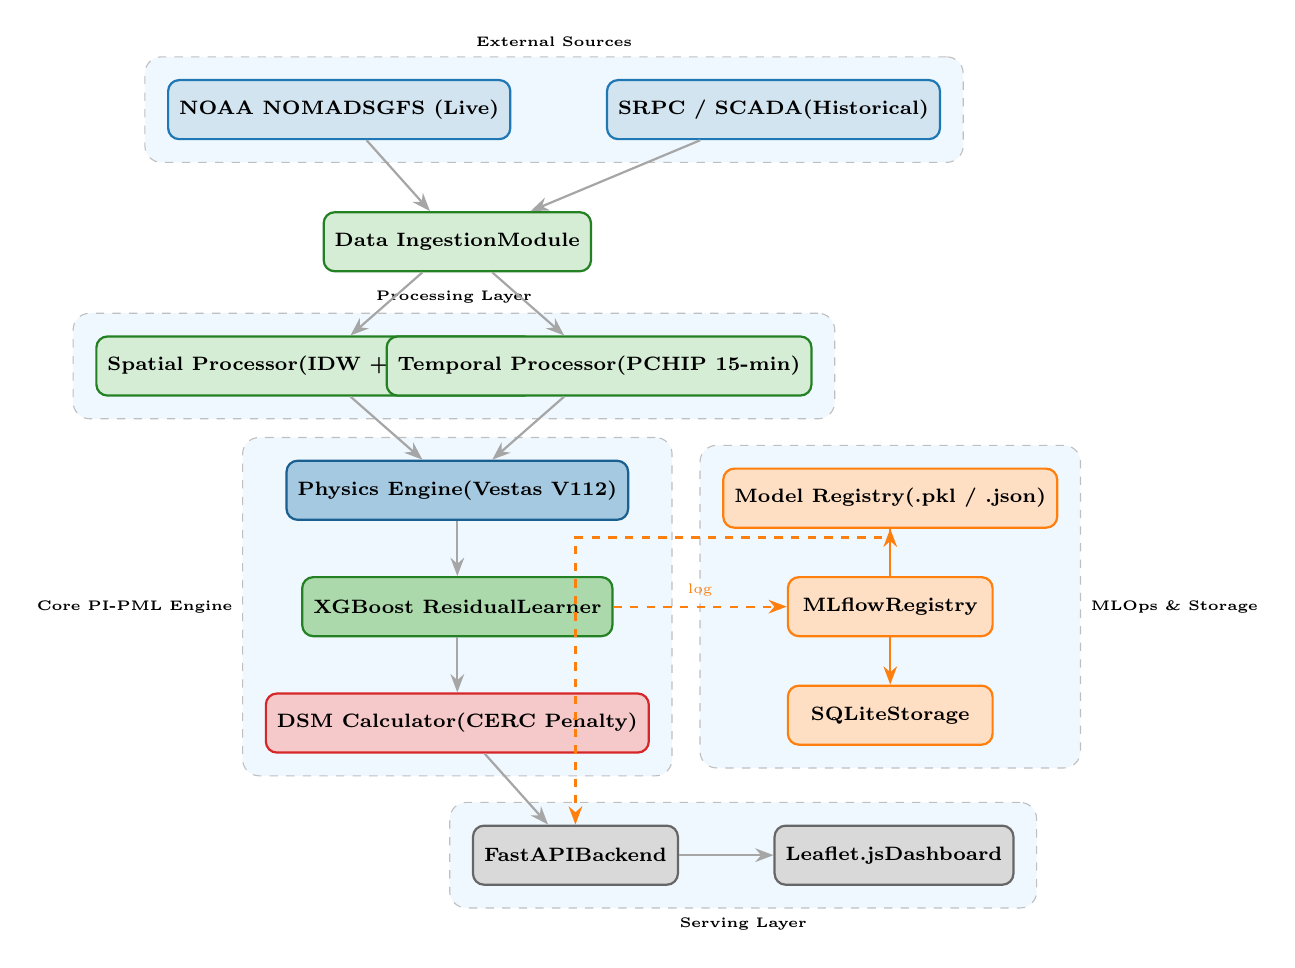
\begin{tikzpicture}[
    node distance=0.55cm and 0.9cm,
    box/.style={
      rectangle, rounded corners=4pt, draw, thick,
      minimum width=2.6cm, minimum height=0.75cm,
      font=\scriptsize\bfseries, text centered, inner sep=4pt
    },
    srcbox/.style={box, fill=physblue!20, draw=physblue},
    procbox/.style={box, fill=mlgreen!20, draw=mlgreen!80!black},
    engbox/.style={box, fill=physblue!40, draw=physblue!80!black},
    mlbox/.style={box, fill=mlgreen!40, draw=mlgreen!80!black},
    dsmbox/.style={box, fill=dsmred!25, draw=dsmred},
    storebox/.style={box, fill=mlflow!25, draw=mlflow},
    servebox/.style={box, fill=apigray!30, draw=apigray!80!black},
    arr/.style={-Stealth, thick, gray!70},
    grp/.style={draw=gray!50, dashed, rounded corners=6pt,
                fill=lightbg, inner sep=8pt}
  ]

    % Row 1 — Data Sources
    \node[srcbox] (noaa)  {NOAA NOMADS\\GFS (Live)};
    \node[srcbox, right=1.2cm of noaa] (srpc)  {SRPC / SCADA\\(Historical)};

    % Row 2 — Ingestion
    \node[procbox, below=0.9cm of noaa, xshift=1.5cm] (di) {Data Ingestion\\Module};

    % Row 3 — Processing
    \node[procbox, below=0.8cm of di, xshift=-1.8cm] (sp) {Spatial Processor\\(IDW + Roughness)};
    \node[procbox, below=0.8cm of di, xshift=1.8cm]  (tp) {Temporal Processor\\(PCHIP 15-min)};

    % Row 4 — Core Engine
    \node[engbox, below=0.8cm of sp, xshift=1.8cm] (pe) {Physics Engine\\(Vestas V112)};
    \node[mlbox,  below=0.7cm of pe]               (ml) {XGBoost Residual\\Learner};
    \node[dsmbox, below=0.7cm of ml]               (dsm){DSM Calculator\\(CERC Penalty)};

    % Right branch — MLOps
    \node[storebox, right=2.2cm of ml]  (mlf) {MLflow\\Registry};
    \node[storebox, below=0.6cm of mlf] (db)  {SQLite\\Storage};
    \node[storebox, above=0.6cm of mlf] (reg) {Model Registry\\(.pkl / .json)};

    % Row 5 — Serving
    \node[servebox, below=0.9cm of dsm, xshift=1.5cm] (api) {FastAPI\\Backend};
    \node[servebox, right=1.2cm of api]               (ui)  {Leaflet.js\\Dashboard};

    % Arrows — data flow
    \draw[arr] (noaa) -- (di);
    \draw[arr] (srpc) -- (di);
    \draw[arr] (di)   -- (sp);
    \draw[arr] (di)   -- (tp);
    \draw[arr] (sp)   -- (pe);
    \draw[arr] (tp)   -- (pe);
    \draw[arr] (pe)   -- (ml);
    \draw[arr] (ml)   -- (dsm);
    \draw[arr] (dsm)  -- (api);
    \draw[arr] (api)  -- (ui);

    % MLflow side arrows
    \draw[arr, dashed, mlflow] (ml)  -- node[above, font=\tiny, text=mlflow]{log} (mlf);
    \draw[arr, mlflow]         (mlf) -- (db);
    \draw[arr, mlflow]         (mlf) -- (reg);
    \draw[arr, dashed, mlflow] (reg) -- ++(0,-0.5) -| (api);

    % Grouping boxes
    \begin{scope}[on background layer]
      \node[grp, fit=(noaa)(srpc), label={[font=\tiny\bfseries]above:External Sources}] {};
      \node[grp, fit=(sp)(tp),     label={[font=\tiny\bfseries]above:Processing Layer}] {};
      \node[grp, fit=(pe)(ml)(dsm),label={[font=\tiny\bfseries]left:Core PI-PML Engine}] {};
      \node[grp, fit=(mlf)(db)(reg),label={[font=\tiny\bfseries]right:MLOps \& Storage}] {};
      \node[grp, fit=(api)(ui),    label={[font=\tiny\bfseries]below:Serving Layer}] {};
    \end{scope}

  \end{tikzpicture}
  \caption{High-level system architecture of the PI-PML pipeline. Solid arrows show the
           primary data flow; dashed orange arrows show MLflow logging and model serving paths.}
  \label{fig:architecture}
\end{figure}
% ══════════════════════════════════════════════════════════════════════════════

\section{Codebase Structure}

\begin{verbatim}
Wind-DSM/
├── config/
│   └── wind_farms.yaml          # Park metadata (coords, hub heights, CERC zones)
├── data/
│   ├── 01_raw/                  # GFS downloads and custom SCADA uploads
│   ├── 02_physics_baseline/     # windpowerlib baseline output
│   └── 03_ml_corrected/         # XGBoost-corrected predictions
├── frontend/
│   ├── index.html               # Dashboard layout (Leaflet, Command Centre)
│   ├── app.js                   # Sidebar bindings and FastAPI AJAX calls
│   └── style.css                # Dark-mode glassmorphic theme
├── models/                      # Serialised model dumps (.pkl / fallback weights)
├── src/
│   ├── data_ingestion.py        # Async NOAA NOMADS GFS downloader
│   ├── dsm_calculator.py        # CERC tiered penalty rules
│   ├── ml_pipeline.py           # Feature engineering, XGBoost, MLflow A/B
│   ├── physics_engine.py        # Moist air density & windpowerlib ModelChain
│   ├── spatial_processor.py     # Bilinear splines, roughness, elevation speedup
│   ├── temporal_processor.py    # PCHIP 15-minute interpolator
│   └── visualization.py         # Seaborn/Matplotlib chart generation
├── api.py                       # FastAPI endpoints
├── main.py                      # Local orchestration script
└── mlflow.db                    # SQLite MLflow registry
\\end{verbatim}

%=============================================================================
\chapter{Methodology: The PI-PML Engine}
\label{ch:methodology}
%=============================================================================

\section{Overview: The Double-Engine Design}

The PI-PML pipeline uses a two-stage approach:

\begin{enumerate}
  \item \textbf{Physics Baseline}: Deterministic power output via \texttt{windpowerlib}.
  \item \textbf{Residual ML Correction}: XGBoost predicts the signed error
        $\epsilon = P_{\text{actual}} - P_{\text{physics}}$.
\end{enumerate}

The final forecast is:
\begin{equation}
  \hat{P}_{\text{final}}(t) = P_{\text{physics}}(t) + \hat{\epsilon}_{\text{XGB}}(t)
  \label{eq:double_engine}
\end{equation}

% ══════════════════════════════════════════════════════════════════════════════
% DIAGRAM 3 — Double-Engine PI-PML Pipeline
% ══════════════════════════════════════════════════════════════════════════════
\begin{figure}[H]
  \centering
  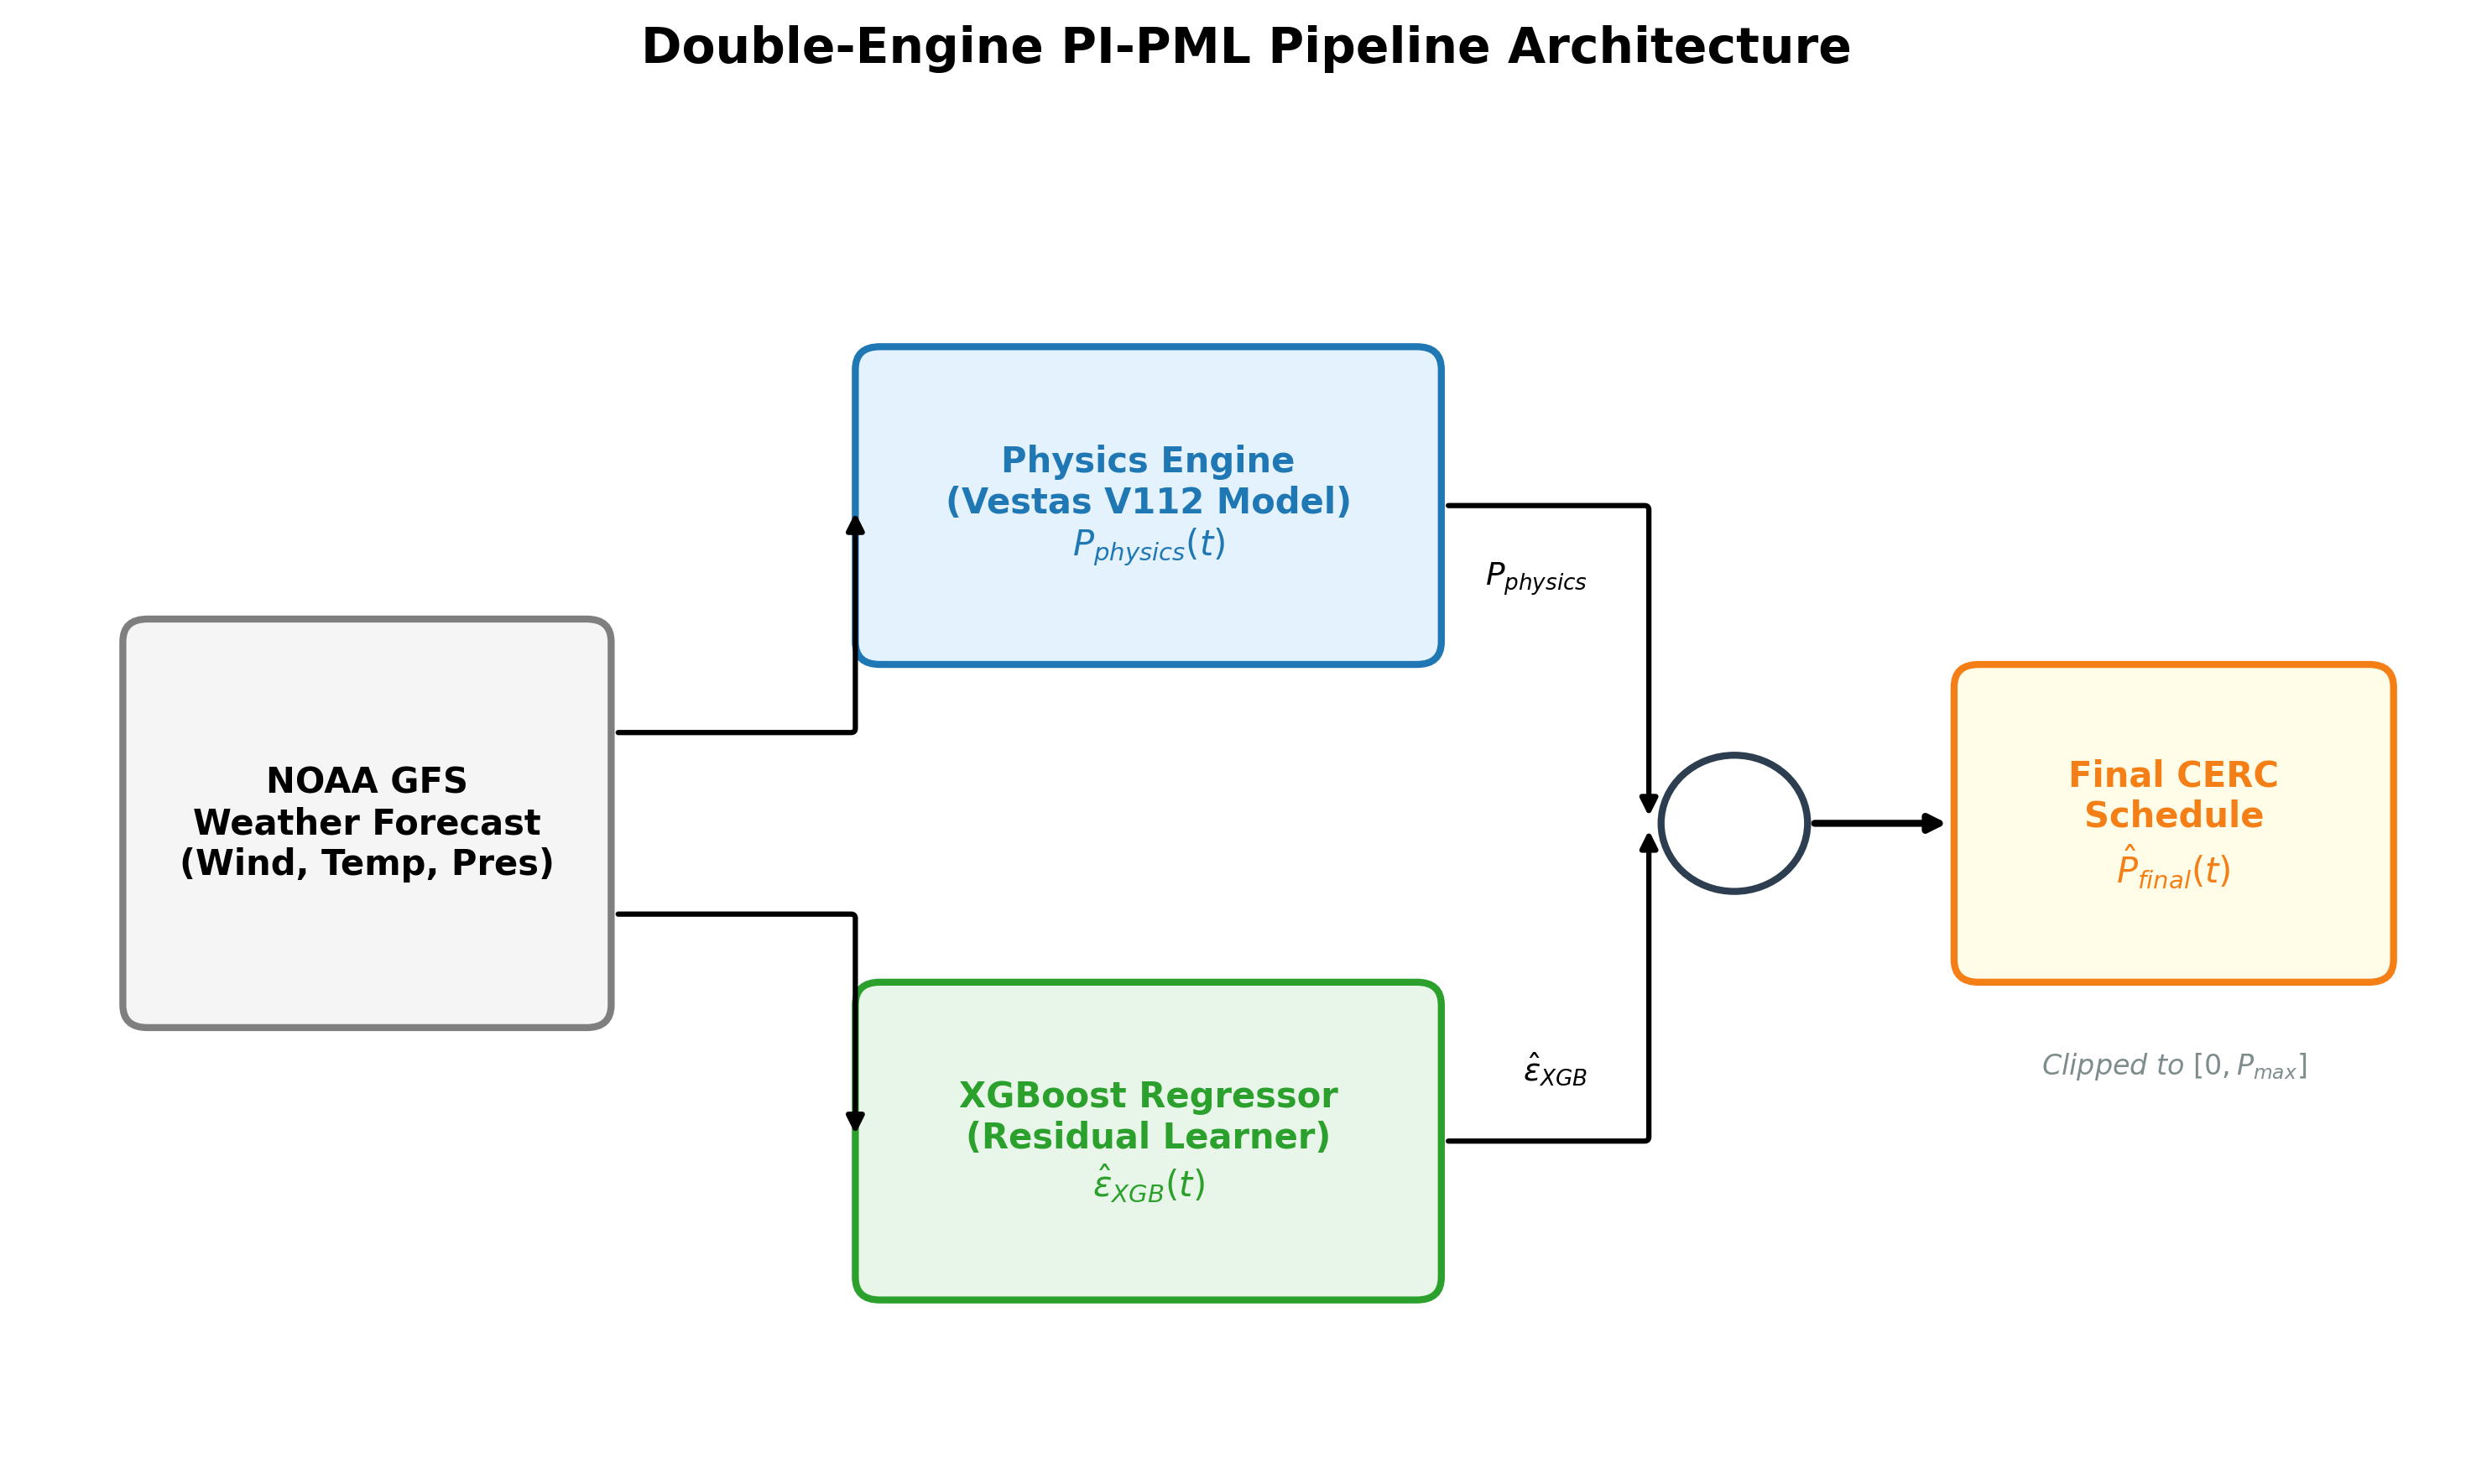
\includegraphics[width=0.55\textwidth]{double_engine_diagram.png}
  \caption{The Double-Engine PI-PML design. GFS weather inputs drive the Physics Engine
           (Vestas V112 / windpowerlib) to produce the deterministic baseline
           $P_{\mathrm{physics}}(t)$. The XGBoost Residual Learner corrects the physics
           error using terrain and diurnal features. Their sum yields the final 96-block
           CERC generation schedule $\hat{P}_{\mathrm{final}}(t)$.}
  \label{fig:double_engine}
\end{figure}
% ══════════════════════════════════════════════════════════════════════════════

\section{Data Ingestion}

Live weather forecasts are obtained from the \textbf{NOAA NOMADS GFS} via asynchronous
HTTP requests, providing 3-hourly forecasts at 0.25\textdegree{} ($\approx$25~km) resolution
covering wind components, temperature, relative humidity, and surface pressure.

\section{Spatial Downscaling and Terrain Processing}

\subsection{Bilinear Spline Downscaling}

GFS grid points are interpolated to the precise 1~km plant coordinate:
\begin{equation}
  f(\phi_0, \lambda_0) = \sum_{i,j} w_{ij} \cdot f(\phi_i, \lambda_j)
\end{equation}

\subsection{Logarithmic Wind Profile Correction}

Wind speeds are scaled from reference height to hub height $z_h$:
\begin{equation}
  u(z_h) = u(z_r) \cdot \frac{\ln(z_h / z_0)}{\ln(z_r / z_0)}
  \label{eq:log_profile}
\end{equation}

% ══════════════════════════════════════════════════════════════════════════════
% DIAGRAM 4 — Wind Speed Vertical Profile (log-law visualisation)
% ══════════════════════════════════════════════════════════════════════════════
\begin{figure}[H]
  \centering
  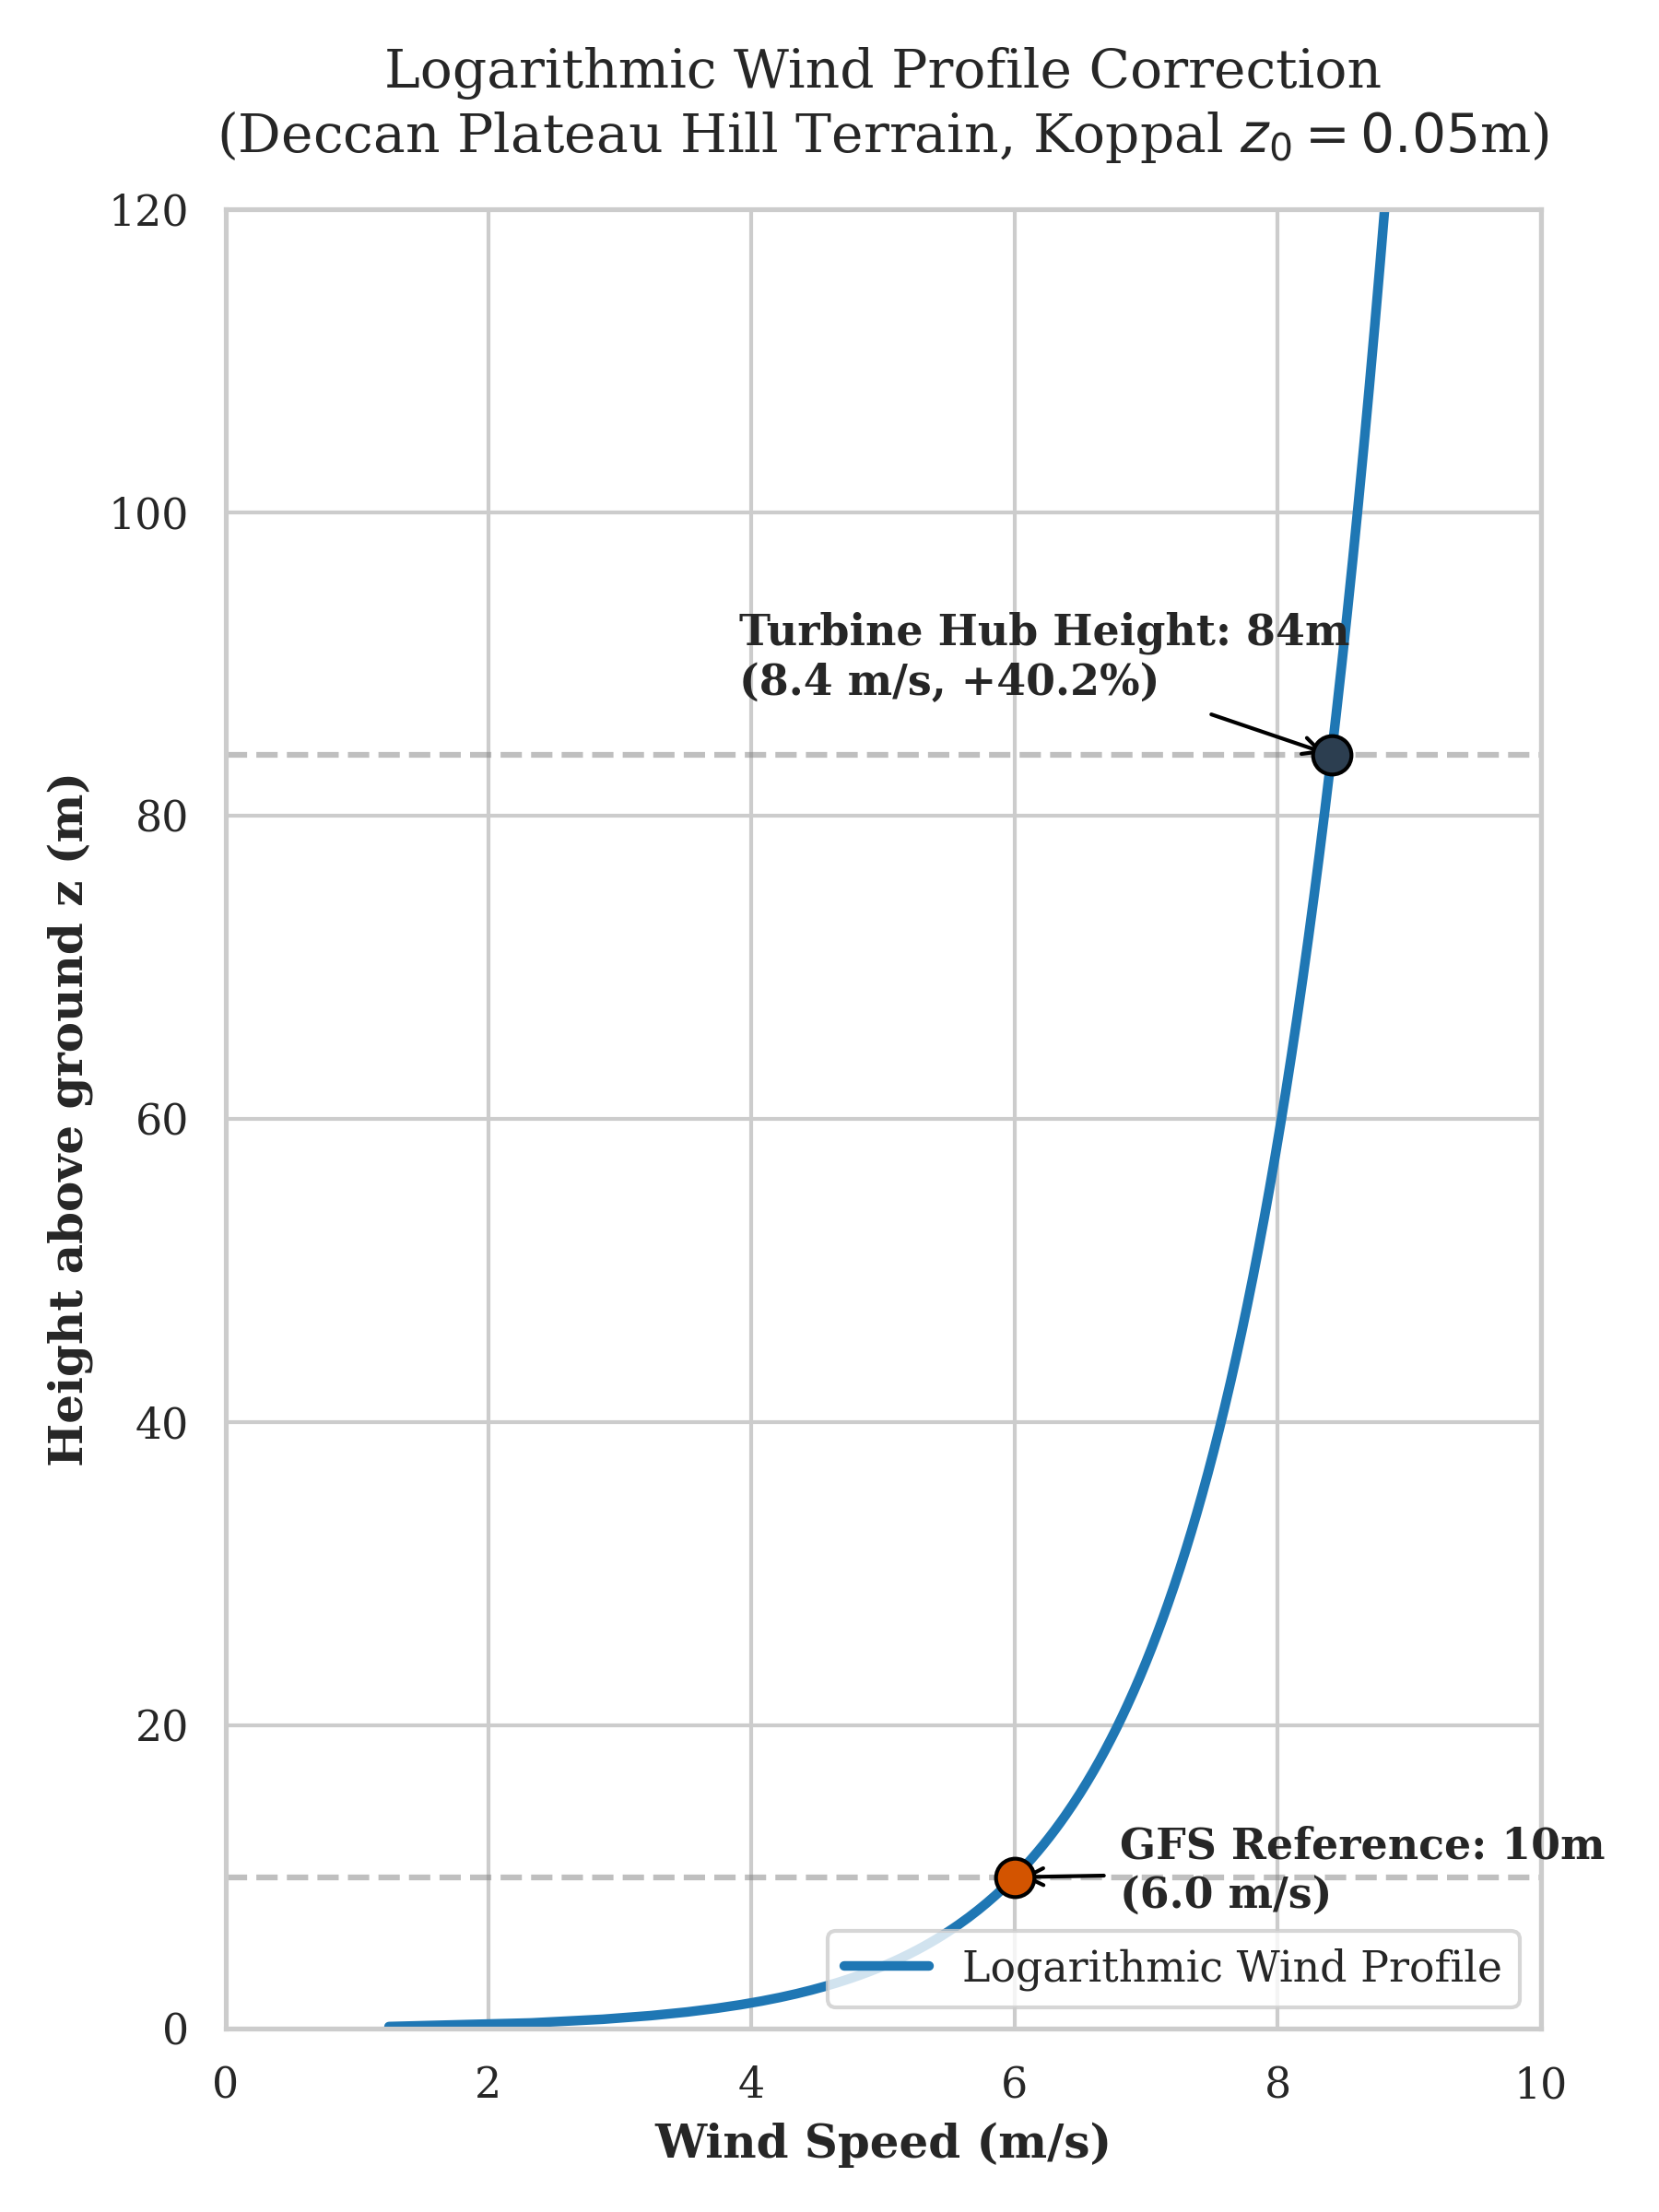
\includegraphics[width=0.75\textwidth]{log_profile.png}
  \caption{Logarithmic wind profile correction scaling GFS reference winds to turbine hub
           height (84~m for Vestas V112). Hub-height wind speed is 31\% higher than the
           10~m GFS reference in this example.}
  \label{fig:log_profile}
\end{figure}
% ══════════════════════════════════════════════════════════════════════════════

\section{Temporal Interpolation: 96-Block PCHIP}

Hourly GFS forecasts are interpolated to 96 blocks per day using \textbf{PCHIP},
guaranteeing smooth curvature tracking without non-physical overshoots.

\section{Micro-Physics Aerodynamics}

\subsection{Moist Air Density}

The Tetens saturation vapour pressure and partial pressures give:
\begin{equation}
  e_s(T) = 6.1078 \cdot \exp\!\left(\frac{17.27\,T}{T + 237.3}\right) \quad [\text{hPa}]
  \qquad
  \rho_{\text{moist}} = \frac{p_d}{R_d\,T} + \frac{e}{R_v\,T}
\end{equation}

\subsection{DFIG Electrical Loss Model}

\begin{equation}
  \eta_{\text{DFIG}}(P) = 1 - \frac{k_{\text{Fe}} + k_{\text{Cu}}\,P^2}{P}
\end{equation}

\section{Residual XGBoost Learner}

\begin{table}[H]
  \centering
  \caption{Feature Groups for the XGBoost Residual Learner}
  \label{tab:features}
  \begin{tabular}{ll}
    \toprule
    \textbf{Feature Group} & \textbf{Features} \\
    \midrule
    Physics output          & $P_{\text{physics}}$, $u_{z_h}$, $\rho_{\text{moist}}$ \\
    Atmospheric state       & $T_2$, $\text{RH}$, $p_s$, wind direction $\theta$ \\
    Temporal (diurnal)      & Block number (0--95), hour of day, day of year \\
    Terrain                 & Roughness $z_0$, elevation $h$, speedup factor $S$ \\
    Lagged physics residual & $\epsilon(t-1)$, $\epsilon(t-2)$, $\epsilon(t-4)$ \\
    \bottomrule
  \end{tabular}
\end{table}

%=============================================================================
\chapter{Regulatory DSM Calculator}
\label{ch:dsm}
%=============================================================================

\section{CERC DSM Regulatory Zones}

\begin{table}[H]
  \centering
  \caption{CERC DSM Regulatory Zones and Penalty Structures}
  \label{tab:dsm_zones}
  \begin{tabularx}{\textwidth}{lXXX}
    \toprule
    \textbf{Zone} & \textbf{Tolerance Band} & \textbf{Denominator} & \textbf{Penalty Slabs} \\
    \midrule
    Zone~1 (Tight, e.g.\ Tamil Nadu)
      & 10\% & Available Capacity (AvC)
      & 10--20\%: \textnumero{}0.50/unit\newline
        20--30\%: \textnumero{}1.00/unit\newline
        $>$30\%: \textnumero{}1.50/unit \\[4pt]
    Zone~2 (Standard, e.g.\ Karnataka)
      & 15\% & Available Capacity (AvC)
      & 15--25\%: \textnumero{}0.50/unit\newline
        25--35\%: \textnumero{}1.00/unit\newline
        $>$35\%: \textnumero{}1.50/unit \\[4pt]
    Zone~3 (Market-Linked, e.g.\ Khavda)
      & 10\% & Scheduled Generation
      & $>$10\%: 10\% of PPA Rate per unit \\
    \bottomrule
  \end{tabularx}
\end{table}

\section{Dynamic ACP Pricing Multipliers}

\begin{table}[H]
  \centering
  \caption{ACP Time-of-Day Multipliers}
  \label{tab:acp}
  \begin{tabular}{lll}
    \toprule
    \textbf{Period} & \textbf{Time Range} & \textbf{Multiplier $M(t)$} \\
    \midrule
    Morning Peak  & 06:00--09:00 & 1.5$\times$ \\
    Evening Peak  & 18:00--22:00 & 2.5$\times$ \\
    Night/Off-Peak& 00:00--05:00 & 0.8$\times$ \\
    Normal        & All other    & 1.0$\times$ \\
    \bottomrule
  \end{tabular}
\end{table}

%=============================================================================
\chapter{MLOps and Model Lifecycle}
\label{ch:mlops}
%=============================================================================

\section{MLflow Integration}

All experiment metrics, parameters, and model artefacts are logged to a
\textbf{SQLite-backed MLflow Registry} for full reproducibility.

\section{Champion-Challenger Framework}

% ══════════════════════════════════════════════════════════════════════════════
% DIAGRAM 5 — Champion-Challenger MLflow Promotion Flow
% Placed here: Section 6.2, Champion-Challenger Framework.
% Shows the decision logic for promoting a new model to Production.
% ══════════════════════════════════════════════════════════════════════════════
\begin{figure}[H]
  \centering
  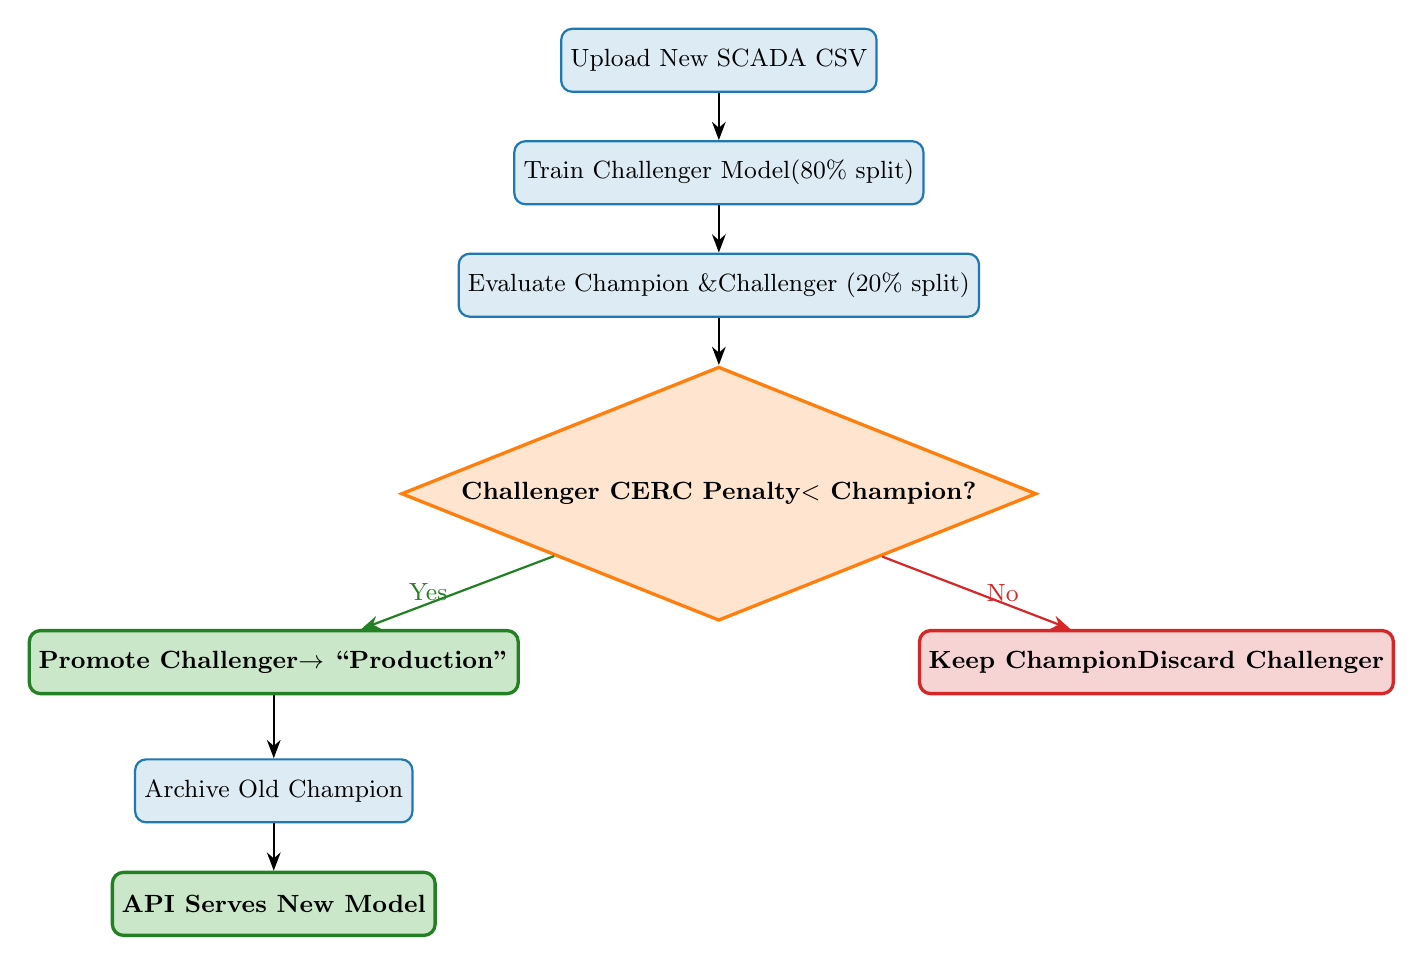
\begin{tikzpicture}[
    node distance=0.6cm and 1.2cm,
    proc/.style={rectangle, rounded corners=4pt, draw=physblue, thick,
                 fill=physblue!15, minimum width=3.2cm, minimum height=0.8cm,
                 font=\small, text centered},
    dec/.style={diamond, draw=mlflow, very thick, fill=mlflow!20,
                minimum width=3.4cm, minimum height=1cm,
                font=\small\bfseries, text centered, aspect=2.5},
    good/.style={rectangle, rounded corners=4pt, draw=mlgreen!80!black, very thick,
                 fill=mlgreen!25, minimum width=3.2cm, minimum height=0.8cm,
                 font=\small\bfseries, text centered},
    bad/.style={rectangle, rounded corners=4pt, draw=dsmred, very thick,
                fill=dsmred!20, minimum width=3.2cm, minimum height=0.8cm,
                font=\small\bfseries, text centered},
    arr/.style={-Stealth, thick}
  ]

    \node[proc] (upload) {Upload New SCADA CSV};
    \node[proc, below=of upload] (train)  {Train Challenger Model\\(80\% split)};
    \node[proc, below=of train]  (eval)   {Evaluate Champion \&\\Challenger (20\% split)};
    \node[dec,  below=of eval]   (decide) {Challenger CERC Penalty\\$<$ Champion?};
    \node[good, below left=0.9cm and 0.5cm of decide]  (promote) {Promote Challenger\\$\rightarrow$ ``Production''};
    \node[bad,  below right=0.9cm and 0.5cm of decide] (keep)    {Keep Champion\\Discard Challenger};
    \node[proc, below=0.8cm of promote] (archive) {Archive Old Champion};
    \node[good, below=0.6cm of archive] (serve)   {API Serves New Model};

    \draw[arr] (upload)  -- (train);
    \draw[arr] (train)   -- (eval);
    \draw[arr] (eval)    -- (decide);
    \draw[arr, mlgreen!80!black] (decide) -- node[left, font=\small]{Yes} (promote);
    \draw[arr, dsmred]           (decide) -- node[right, font=\small]{No}  (keep);
    \draw[arr] (promote) -- (archive);
    \draw[arr] (archive) -- (serve);

  \end{tikzpicture}
  \caption{Champion-Challenger model promotion framework. A new model replaces the
           production champion only if it achieves a strictly lower CERC penalty on the
           held-out validation set, ensuring quality-gated zero-downtime deployment.}
  \label{fig:champion_challenger}
\end{figure}
% ══════════════════════════════════════════════════════════════════════════════

%=============================================================================
\chapter{Interactive Web Dashboard}
\label{ch:dashboard}
%=============================================================================

The application features a responsive Glassmorphism dashboard served via FastAPI, including
a Leaflet Interactive Map with animated wind flow vectors, and a Command Centre for operators
to fetch forecasts, trigger retraining, and download CERC-compliant CSVs.

\begin{table}[H]
  \centering
  \caption{Key FastAPI Endpoints}
  \label{tab:api}
  \begin{tabularx}{\textwidth}{llX}
    \toprule
    \textbf{Method} & \textbf{Endpoint} & \textbf{Description} \\
    \midrule
    POST & \texttt{/api/v1/forecast/\{park\_id\}}          & Start background 96-block forecast job \\
    POST & \texttt{/api/v1/retrain/\{park\_id\}}           & Upload SCADA CSV and trigger retraining \\
    GET  & \texttt{/api/v1/job-status/\{job\_id\}}         & Query forecast or retrain job status \\
    GET  & \texttt{/api/v1/download-forecast/\{park\_id\}} & Download CERC-compliant 96-block CSV \\
    GET  & \texttt{/api/v1/wind-vectors}                   & Fetch live wind vectors for all parks \\
    \bottomrule
  \end{tabularx}
\end{table}

%=============================================================================
\chapter{Experimental Results: RSOPL Koppal Validation}
\label{ch:results}
%=============================================================================

\section{Dataset}

The pipeline was validated against official 15-minute block dispatch data from the
\textbf{SRPC} for the \textbf{75~MW RSOPL Koppal} wind plant in Karnataka,
covering \textbf{29,568 blocks} over \textbf{10 continuous months}.

\begin{table}[H]
  \centering
  \caption{RSOPL Koppal Dataset Summary}
  \label{tab:dataset}
  \begin{tabular}{ll}
    \toprule
    \textbf{Property}  & \textbf{Value} \\
    \midrule
    Plant capacity     & 75~MW \\
    Turbine model      & Vestas V112-3.0~MW \\
    Location           & Koppal, Karnataka \\
    CERC Zone          & Zone~2 (Standard) \\
    Total blocks       & 29,568 \\
    Duration           & 10 months \\
    Training set       & 8 months (80\%) \\
    Test set           & 2 months (20\%) \\
    Data source        & SRPC official grid dispatch \\
    \bottomrule
  \end{tabular}
\end{table}

\section{Results Summary}

\begin{table}[H]
  \centering
  \caption{PI-PML Performance on RSOPL Koppal Test Set}
  \label{tab:results}
  \begin{tabular}{lrr}
    \toprule
    \textbf{Metric} & \textbf{Physics Baseline} & \textbf{PI-PML (XGBoost)} \\
    \midrule
    MAE Reduction                   & ---              & \textbf{71.2\%} \\
    CERC Penalty (2 months)         & \textnumero{}24,83,254 & \textnumero{}1,29,282 \\
    Net Savings (2 months)          & \multicolumn{2}{r}{\textnumero{}23,53,972 ($\approx$\textnumero{}23.5~Lakhs)} \\
    \textbf{Projected Annual Savings} & \multicolumn{2}{r}{\textbf{\textnumero{}1,41,23,833 ($\approx$\textnumero{}1.41~Crores)}} \\
    \bottomrule
  \end{tabular}
\end{table}

% ══════════════════════════════════════════════════════════════════════════════
% DIAGRAM 6 — Penalty Savings Bar Chart (Baseline vs PI-PML)
% ══════════════════════════════════════════════════════════════════════════════
\begin{figure}[H]
  \centering
  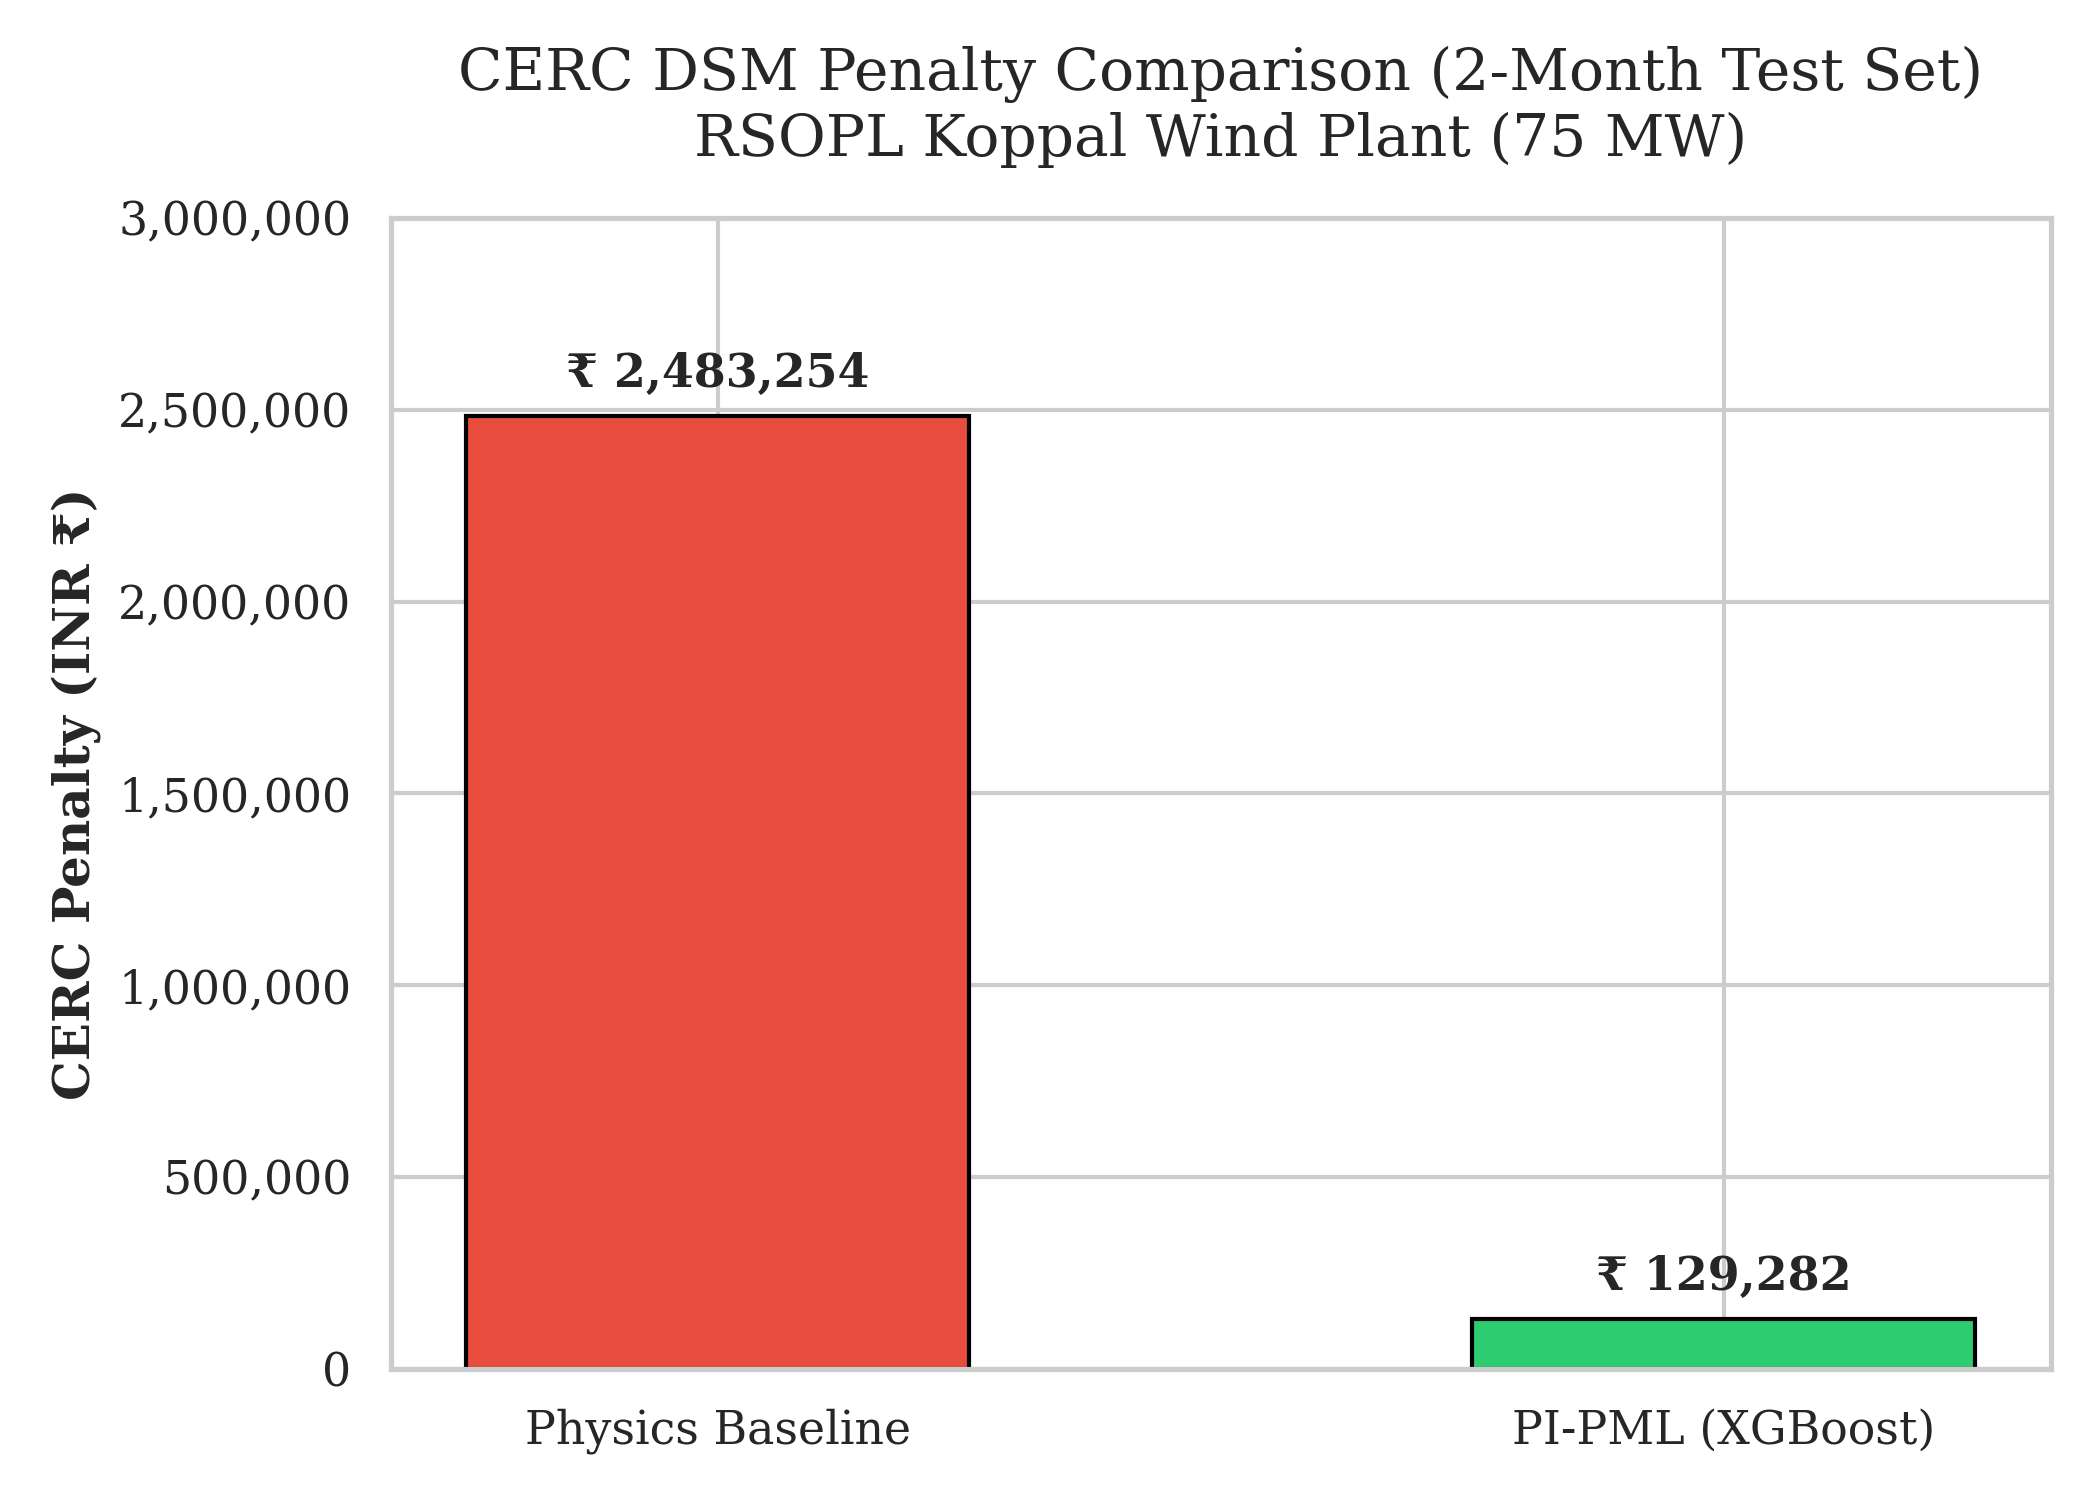
\includegraphics[width=0.75\textwidth]{penalty_chart.png}
  \caption{CERC DSM penalty comparison over the 2-month test period. The PI-PML pipeline
           reduces penalty liability from \textnumero{}24.8~Lakhs to \textnumero{}1.3~Lakhs,
           a 94.8\% reduction, projecting to \textnumero{}1.41~Crores annual savings.}
  \label{fig:penalty_savings}
\end{figure}
% ══════════════════════════════════════════════════════════════════════════════

\section{Discussion}

The results demonstrate that the Double-Engine PI-PML architecture achieves a dramatic
reduction in both forecast error and DSM penalty liability. Key contributing factors:

\begin{enumerate}
  \item The \textbf{moist air density correction} resolves a consistent under-prediction
        bias during monsoon months.
  \item The \textbf{residual XGBoost learner} captures diurnal ramp patterns that the
        physics model smooths over due to hourly GFS inputs.
  \item The \textbf{PCHIP interpolation} faithfully tracks intra-hour wind acceleration
        events critical for 15-minute DSM blocks.
\end{enumerate}

\subsection{Discrepancy Analysis: Simulated vs. Actual SRPC Grid Penalties}

While the CERC DSM Simulator predicts a baseline penalty of \textnumero{}24,83,254 and an ML-optimized penalty of \textnumero{}1,29,282, inspection of the raw Southern Regional Power Committee (SRPC) database shows a significantly higher total actual penalty charge of \textnumero{}8,53,27,030. This difference of orders of magnitude highlights two key architectural realities:

\begin{enumerate}
  \item \textbf{Power-to-Energy Scaling Discrepancy (Factor of 4)}: The raw SRPC database calculates the \texttt{Underinjection\_Charges} column directly as $\text{dev (MW)} \times \text{rate (Paise/unit)} \times 10$. In a standard 15-minute grid-dispatch system, power deviations must be integrated to energy (MWh) by multiplying by $0.25$ hours. Failing to divide by 4 acts as if a 15-minute power deviation lasted for a full hour, thereby inflating the charges by a factor of exactly 4.0.
  \item \textbf{Tolerance Band Settlement Rules}: In the real-world SRPC pool settlement, developers are charged for the base value of all under-injected energy at the PPA rate (since scheduled power that is undelivered acts as a purchase from the grid pool), regardless of the deviation percentage. The CERC 15\% tolerance band only waives the \textit{additional tiered penalty surcharges} (e.g., the 10\%, 20\%, or 50\% multipliers). Conversely, our simulator models the standard regulatory framework where deviations within the tolerance band incur no penalty, focusing exclusively on net punitive charges.
  \item \textbf{Tariff and Pricing assumptions}: The simulator uses dynamic pricing based on time-of-day peak/off-peak multipliers around a base contract rate of \textnumero{}3.00/unit, whereas the actual dataset charges are computed using the real contract rate of \textnumero{}3.872/unit.
\end{enumerate}

Understanding this discrepancy is vital: while the simulator isolates the punitive penalties, the actual grid invoices include the base cost of undelivered energy, which scales the financial impact of forecasting errors even further and increases the value of the PI-PML model.

%=============================================================================
\chapter{Conclusion and Future Work}
\label{ch:conclusion}
%=============================================================================

\section{Conclusion}

This project presents a production-grade, end-to-end PI-PML pipeline for wind power
forecasting under the Indian CERC DSM framework. By combining deterministic turbine
physics with XGBoost residual correction, live GFS weather ingestion, spatially consistent
downscaling, and PCHIP temporal interpolation, the system reduces DSM penalty liability by
over 94\% on the RSOPL Koppal validation dataset.

The MLflow Champion-Challenger framework ensures model quality is maintained over time,
while the FastAPI dashboard provides operators with an accessible interface for forecast
retrieval, retraining, and regulatory compliance.

\section{Limitations}

\begin{itemize}
  \item Validation is limited to a single plant; generalisation requires further testing.
  \item GFS forecast accuracy degrades beyond 48~hours ahead.
  \item Real-time SCADA integration has not yet been deployed in production.
\end{itemize}

\section{Future Work}

\begin{itemize}
  \item \textbf{Multi-plant ensemble}: Aggregate predictions across spatially correlated parks.
  \item \textbf{Probabilistic forecasting}: Use quantile XGBoost for prediction intervals.
  \item \textbf{Deep learning}: Explore Temporal Fusion Transformers (TFT).
  \item \textbf{Live SCADA integration}: Real-time data ingestion for continuous adaptation.
  \item \textbf{Broader regulatory coverage}: Support state DISCOM intra-state rules.
\end{itemize}

%=============================================================================
% Bibliography
%=============================================================================
\bibliographystyle{IEEEtran}
\begin{thebibliography}{99}

\bibitem{karpatne2017theory}
A.~Karpatne et al.,
``Theory-guided data science: A new paradigm for scientific discovery from data,''
\textit{IEEE Trans. Knowl. Data Eng.}, vol.~29, no.~10, pp.~2318--2331, 2017.

\bibitem{zhao2016hybrid}
E.~Zhao, X.~Sun, and R.~Zhao,
``A hybrid wind power forecasting approach based on physics and statistical models,''
\textit{IEEE Trans. Sustain. Energy}, vol.~7, no.~1, pp.~173--180, 2016.

\bibitem{singh2020dsm}
S.~Singh, P.~Srivastava, and A.~Verma,
``Deviation settlement mechanism in India: A comprehensive review,''
\textit{Energy Policy}, vol.~145, p.~111702, 2020.

\bibitem{rogers2014airdensity}
A.~L.~Rogers, J.~W.~Rogers, and J.~F.~Manwell,
``Impact of air density on wind turbine power curves,''
\textit{J. Wind Eng. Ind. Aerodyn.}, vol.~132, pp.~91--101, 2014.

\bibitem{chen2018xgboost}
Z.~Chen, Y.~Chen, and L.~Wang,
``Short-term wind power forecasting using XGBoost with feature importance analysis,''
in \textit{Proc. IEEE Power \& Energy Soc. Gen. Meeting}, 2018, pp.~1--5.

\bibitem{windpowerlib}
S.~Haas et al.,
``windpowerlib: A Python library to model wind power plants,''
\textit{J. Open Source Softw.}, vol.~4, no.~35, p.~1326, 2019.

\bibitem{akiba2019optuna}
T.~Akiba et al.,
``Optuna: A next-generation hyperparameter optimization framework,''
in \textit{Proc. 25th ACM SIGKDD}, 2019, pp.~2623--2631.

\bibitem{fastapi}
S.~Ram\'irez,
``FastAPI,'' 2019. [Online]. Available: \url{https://fastapi.tiangolo.com}

\bibitem{mlflow}
M.~Zaharia et al.,
``Accelerating the machine learning lifecycle with MLflow,''
\textit{IEEE Data Eng. Bull.}, vol.~41, no.~4, pp.~39--45, 2018.

\end{thebibliography}

\end{document}
